\documentclass[border=4pt]{standalone}
\usepackage{fontspec}
\usepackage{amsmath}
\usepackage{unicode-math}
\setmainfont{Latin Modern Roman}
\setmathfont{Latin Modern Math}
\usepackage{pgfplots}
\usepackage{pgfplotstable}
\pgfplotsset{compat=1.18}
\usepackage{tkz-euclide}
\usetikzlibrary{arrows.meta,calc,angles,quotes,patterns,3d,backgrounds}
\definecolor{ink}{HTML}{123428}
\definecolor{asy}{HTML}{475569}
\definecolor{mint}{HTML}{86e0bd}
\tikzset{asym/.style={asy, line width=0.9pt, dash pattern=on 5pt off 3.5pt},
         guide/.style={gray!70, line width=0.6pt, densely dotted},
         dot/.style={circle, inner sep=0pt, minimum size=5pt, draw=white, line width=0.5pt},
         odot/.style={circle, inner sep=0pt, minimum size=5.5pt, fill=white, line width=1pt},
         lab/.style={font=\footnotesize, inner sep=1.5pt, text=ink}}
\begin{document}
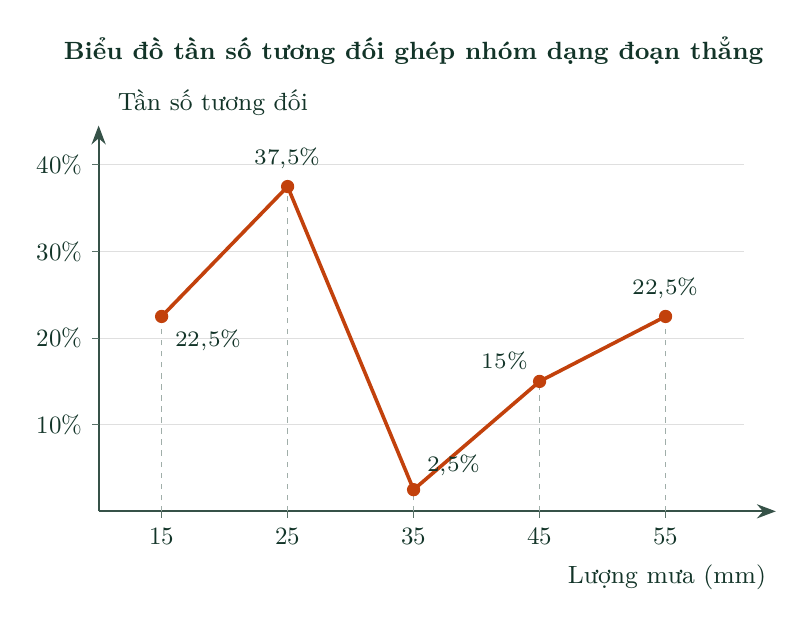
\begin{tikzpicture}
\draw[gray!25, line width=0.4pt] (0,1.100) -- (8.200,1.100);
\draw[gray!25, line width=0.4pt] (0,2.200) -- (8.200,2.200);
\draw[gray!25, line width=0.4pt] (0,3.300) -- (8.200,3.300);
\draw[gray!25, line width=0.4pt] (0,4.400) -- (8.200,4.400);
\draw[ink!85, line width=0.7pt, -{Stealth[length=2.4mm]}] (0,0) -- (8.600,0);
\draw[ink!85, line width=0.7pt, -{Stealth[length=2.4mm]}] (0,0) -- (0,4.900);
\draw[ink!40, dash pattern=on 2pt off 2pt] (0.800,0) -- (0.800,2.475);
\draw[ink!40, dash pattern=on 2pt off 2pt] (2.400,0) -- (2.400,4.125);
\draw[ink!40, dash pattern=on 2pt off 2pt] (4.000,0) -- (4.000,0.275);
\draw[ink!40, dash pattern=on 2pt off 2pt] (5.600,0) -- (5.600,1.650);
\draw[ink!40, dash pattern=on 2pt off 2pt] (7.200,0) -- (7.200,2.475);
\draw[color={rgb,255:red,194;green,65;blue,12}, line width=1.3pt] (0.800,2.475) -- (2.400,4.125) -- (4.000,0.275) -- (5.600,1.650) -- (7.200,2.475);
\fill[color={rgb,255:red,194;green,65;blue,12}] (0.800,2.475) circle (2.4pt);
\node[font=\footnotesize, text=ink, below right=2pt] at (0.800,2.475) {$22{,}5\%$};
\draw[ink!70] (0.800,0) -- (0.800,-0.08) node[below, font=\small, text=ink] {$15$};
\fill[color={rgb,255:red,194;green,65;blue,12}] (2.400,4.125) circle (2.4pt);
\node[font=\footnotesize, text=ink, above=3pt] at (2.400,4.125) {$37{,}5\%$};
\draw[ink!70] (2.400,0) -- (2.400,-0.08) node[below, font=\small, text=ink] {$25$};
\fill[color={rgb,255:red,194;green,65;blue,12}] (4.000,0.275) circle (2.4pt);
\node[font=\footnotesize, text=ink, above right=2pt] at (4.000,0.275) {$2{,}5\%$};
\draw[ink!70] (4.000,0) -- (4.000,-0.08) node[below, font=\small, text=ink] {$35$};
\fill[color={rgb,255:red,194;green,65;blue,12}] (5.600,1.650) circle (2.4pt);
\node[font=\footnotesize, text=ink, above left=1pt] at (5.600,1.650) {$15\%$};
\draw[ink!70] (5.600,0) -- (5.600,-0.08) node[below, font=\small, text=ink] {$45$};
\fill[color={rgb,255:red,194;green,65;blue,12}] (7.200,2.475) circle (2.4pt);
\node[font=\footnotesize, text=ink, above=3pt] at (7.200,2.475) {$22{,}5\%$};
\draw[ink!70] (7.200,0) -- (7.200,-0.08) node[below, font=\small, text=ink] {$55$};
\draw[ink!70] (0,1.100) -- (-0.08,1.100) node[left, font=\small, text=ink] {$10\%$};
\draw[ink!70] (0,2.200) -- (-0.08,2.200) node[left, font=\small, text=ink] {$20\%$};
\draw[ink!70] (0,3.300) -- (-0.08,3.300) node[left, font=\small, text=ink] {$30\%$};
\draw[ink!70] (0,4.400) -- (-0.08,4.400) node[left, font=\small, text=ink] {$40\%$};
\node[font=\small, text=ink, anchor=north east] at (8.600,-0.55) {Lượng mưa (mm)};
\node[font=\small, text=ink, anchor=south west] at (0.12,4.900) {Tần số tương đối};
\node[font=\bfseries\small, text=ink] at (4.000,5.850) {Biểu đồ tần số tương đối ghép nhóm dạng đoạn thẳng};
\end{tikzpicture}
\end{document}
